% -*- Index -*-


\chapter{Strategies}
\label{chap:Strategies}

\index{strategy|(}

\IceT contains several parallel image compositing algorithms.  The type of
compositing algorithm to use is selected by choosing a
\index{strategy}\keyterm{strategy}.  This chapter describes the underlying
algorithm of each strategy.  This user's guide will give qualitative
comparisons between the strategies, but for a more quantitative analysis,
see the following paper.

\begin{quote}
  Kenneth Moreland, Brian Wylie, and Constantine Pavlakos.  ``Sort-last
  parallel rendering for viewing extremely large data sets on tile
  displays,'' In \emph{Proceedings of IEEE Symposium on Parallel and
    Large-Data Visualization and Graphics}, October 2001, pp. 85--154.
\end{quote}

A strategy is specified using the \CFunc{icetStrategy} function.

\begin{Table}{3}
  \textC{void }\CFunc{icetStrategy}\textC{(}&\CType{IceTStrategy}&\CArg{strategy}\quad\textC{);}
\end{Table}

The \CArg{strategy} is set to one of the identifiers for the strategies
documented in the following sections of this chapter.  A string documenting
the current strategy can be retrieved with the \CFunc{icetGetStrategyName}
function.

To describe the \IceT compositing algorithms, we will use the example
parallel rendering problem shown in Figure~\ref{fig:ExampleInputs} where 6
processes are each rendering their own piece of a shuttle model to a two
tile display.

\begin{figure}
  \centering
  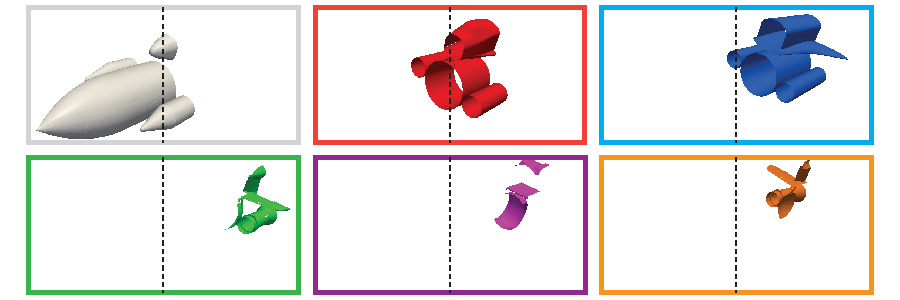
\includegraphics{images/AllInput}
  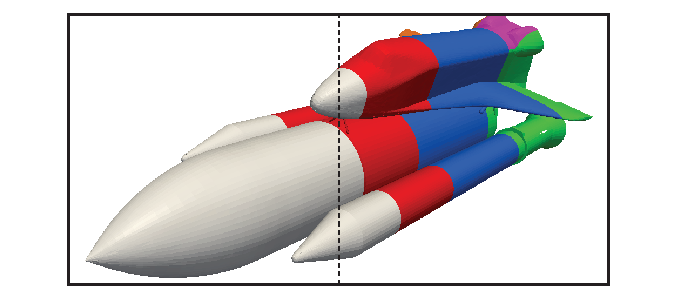
\includegraphics{images/CompositedInput}
  \caption[Example compositing problem.]{An example of six processes
    rendering to two tiles (top) and their composited image (bottom).}
  \label{fig:ExampleInputs}
\end{figure}

In this example, processes are denoted, in no particular order, by the
colors gray, red, blue, green, purple, and orange.  The colors of the
geometry correspond to the process that generated each piece.  Image
boarder colors denote the process that generates and holds that image.
(Apologies to those having troubles resolving the colors due to poor
display or vision deficiencies.  It should not be hard to follow the
descriptions either way.)

\section{Single Image Compositing}

\index{single~image~composite|(}
\index{compositing!single~image|(}

Before discussing the multi-tile image compositing algorithms implemented
by \IceT, we visit the standard single image compositing algorithms.  You
cannot directly select a single image compositing algorithm as a strategy
(most of the multi-tile algorithms work well in ``single-tile'' mode), but
these compositing algorithms are used as ``subroutines'' in some of the
multi-tile algorithms.  A reference to a
\index{single~image~composite~network}\keyterm{single image composite
  network} in the subsequent compositing algorithm descriptions refers to
the algorithms described here.

\subsection{Tree Compositing}

\index{compositing!tree|(}
\index{tree~composite|(}
\index{binary~tree~composite|(}

\IceT internally has two single image composite implementations.  The first
of which is the \keyterm{tree composite} algorithm (sometimes also called
binary tree composite due to its pair-wise grouping).  The basic network
for tree composite is shown in Figure~\ref{fig:BinaryTree}.

\begin{figure}
  \centering
  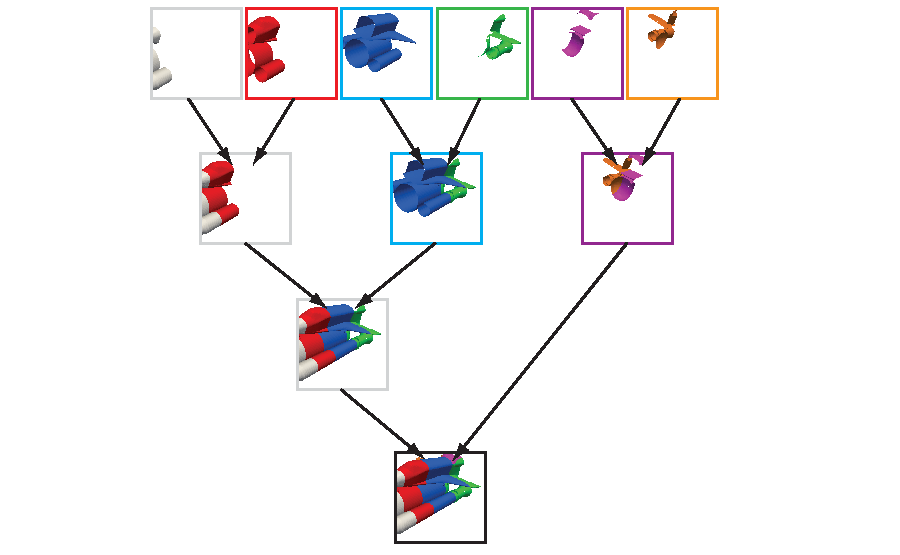
\includegraphics{images/BinaryTree}
  \caption[Tree composite network.]{Tree composite network.  Arrows
    represent the passing of data from one stage to the next.  Processes
    receiving multiple images composite them together.}
  \label{fig:BinaryTree}
\end{figure}

The tree compositing algorithm is organized in stages.  At each stage the
processes pair up.  One of the processes sends its data to its pair and
then drops out of the computation.  The receiving process combines the two
images (using the \index{compositing~operation}compositing operation
described in
Chapter~\ref{sec:Customizing_Compositing:Compositing_Operation}) and
continues to the next stage.  Processing continues until there is only one
image (and one process) remaining.

As just defined, the tree composite algorithm only handles process counts
that are a power of two (that is, the number of processes is equal to $2^i$
for some integer $i$).  \IceT handles non-powers of two gracefully.  At any
stage where the number of processes is not even and one of the processes
cannot be paired, that leftover process does nothing for that stage but
then continues to participate in the next stage.  An example of this can be
seen in the second stage of Figure~\ref{fig:BinaryTree}.

The advantages of tree composite are its regular and efficient data
transfers.  The limiting factor of tree compositing is that at each stage
of the algorithm half of the processes drop out of the computation.  Thus,
for more than a few processes tree compositing provides poor process
utilization.

\index{binary~tree~composite|)}
\index{tree~composite|)}
\index{compositing!tree|)}

\subsection{Binary-Swap Compositing}

\index{compositing!binary~swap|(}
\index{binary~swap~composite|(}

The second single image compositing algorithm used internally by \IceT is
the \keyterm{binary swap} algorithm.  The basic network for binary-swap
composite is shown in Figure~\ref{fig:BinarySwap}

\begin{figure}
  \centering
  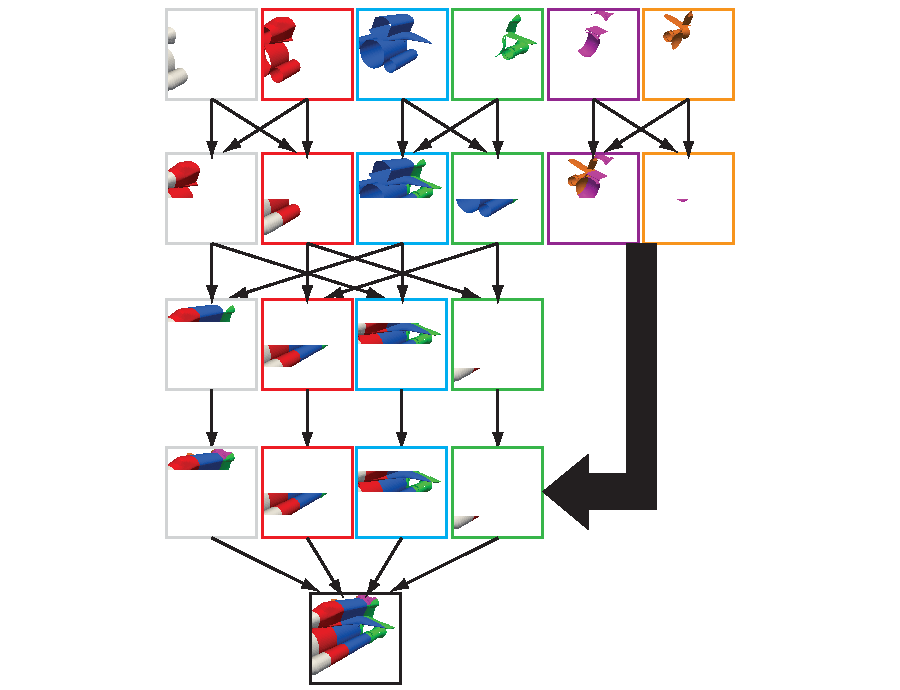
\includegraphics{images/BinarySwap}
  \caption[Binary-swap composite network.]{Binary-swap composite network.
    Arrows represent the passing of data from one stage to the next.
    Processes receiving multiple images composite or stitch them together.
    At most stages each process divides its image data and distributes it.
    The distribution of image data can be inferred from the target images.}
  \label{fig:BinarySwap}
\end{figure}

Like tree compositing, binary swap is organized in stages, and at each
stage the processes pair up.  However, rather than have one process send
all the data to the other, the image space is divided in two and the
processes swap image data so that each process has all the data for part of
the image.  At the next stage, the processes pair up again, but with
different partners that have the same partition of the image.  Processing
continues until each of the $N$ processes have an image $1/N$ the size of
the original image.  At this point, all the processes send their sub-image
to the display processes where the images are stitched together.

As just defined, the binary-swap composite algorithm only handles processes
that are a power of two (that is, the number of processes is equal to $2^i$
for some integer $i$).  Some binary-swap implementations handle non-powers
of two by reducing the problem to the next largest power of two and
dropping the leftover processes, but \IceT handles non-powers of two more
gracefully than that.  Instead, \IceT first finds the largest group of
processes that is a power of two, makes a partition out of them, then finds
the next largest group of processes that remain that is a power of two,
makes a partition out of them, and so on.  Each partition runs binary-swap
independently up to the point where each process has its own piece of data.
At this point, the smaller partitions send their image data to processes of
the larger partitions, dividing up images where necessary.  The largest
partition then finishes the compositing in the normal way by collecting all
of the pieces.

An example of compositing with a non-power of two is given in
Figure~\ref{fig:BinarySwap}.  The six processes are partitioned first into
a group of 4 and then into a group of 2.  After swapping, the processes in
the smaller group send images to the larger group.  In this case, the purple
process sends image data to the gray and blue processes, and the orange
process sends to the red and green processes.

Like tree composite, binary swap exhibits regular and efficient data
transfers.  In addition, binary swap involves the use of all the processes
throughout most of the compositing.  Consequently, binary swap exhibits
very good process utilization and scaling with respect to the number of
processes on which it is run.

The most inefficient part of binary swap is the collection of image
fragments at the end, which is an extra step that tree composite does not
need to take.  Through some empirical studies, we found that the binary
tree algorithm was more efficient than binary swap on less then 8 processes and
less efficient on more than 8 processes.  Consequently, \IceT automatically
switches between the two algorithms based on the amount of processes
involved in the compositing.

\index{binary~swap~composite|)}
\index{compositing!binary~swap|)}

\subsection{Ordered Compositing}

\index{compositing!ordered|(}

In some applications, the order in which images are composited together
makes a difference (see the Volume Rendering section in
Chapter~\ref{sec:Customizing_Compositing:Volume_Rendering}).  The details
on how ordered compositing is achieved is not given here, but the basic
idea for both compositing algorithms is that they first swizzle the
processes so that their order matches the order in which the images need to
be composited together.  When compositing images together, they make sure
to maintain over/under constancy based on the swizzled ranks from the
originating processes.  The networks are also managed such that no two
images are composited that are not directly ``next'' to each other (that
is, there is no image that needs to be inserted between them).

\index{compositing!ordered|)}

\index{compositing!single~image|)}
\index{single~image~composite|)}

\section{Reduce Strategy}
\label{sec:Strategies:Reduce}

\index{strategy!reduce|(}
\index{reduce~strategy|see{strategy, reduce}}
\index{reduce~to~single~tile|see{strategy, reduce}}

An effective strategy implemented in \IceT is the \keyterm{reduce to single
  tile strategy} (or simply the reduce strategy).  In this strategy, the
multi-tile composite problem is efficiently reduced to a set of single
image compositing problems, which are well studied and discussed in the
previous section.  The reduce strategy is selected by calling
\CFunc{icetStrategy} with the \CEnum{ICET\_STRATEGY\_REDUCE} argument.

\begin{figure}
  \centering
  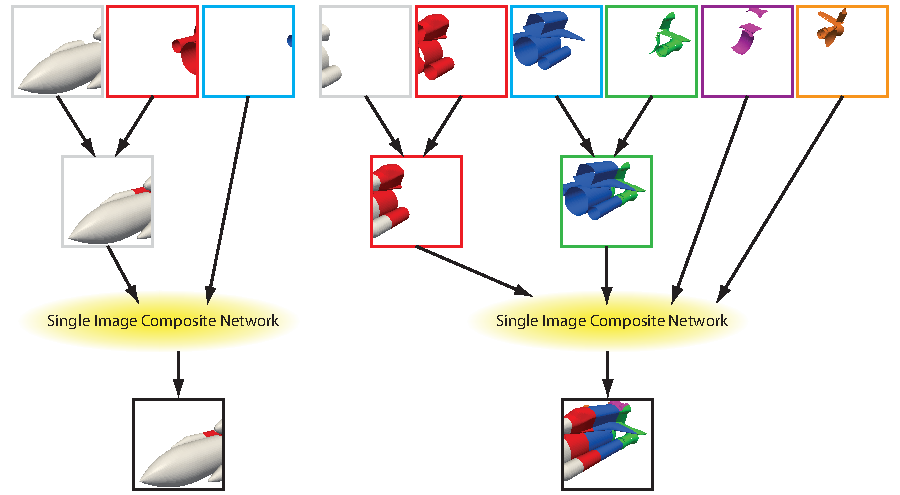
\includegraphics{images/ReduceComposite}
  \caption[Reduce strategy composite network.]{Composite network for reduce
    strategy.  Arrows represent the passing of data from one stage to the
    next.  Processes receiving multiple images composite them together.
    The single image composite network is described in a preceding
    section.}
  \label{fig:ReduceComposite}
\end{figure}

The reduce strategy is performed in two phases.  In the first phase,
processes are partitioned into groups, each of which is responsible for
compositing the image of one of the tiles.  The number of processes
assigned to each tile is proportional to the number of non-empty images
rendered for the corresponding tile.  In the example shown in
Figure~\ref{fig:ReduceComposite} there are a total of 9 non-empty images.
The left tile has 3 of the 9, that is $\frac{1}{3}$, of the images and thus
is assigned $\frac{1}{3} \times 6 = 2$ processes.  Likewise, the right
image is assigned $\frac{2}{3} \times 6 = 4$ processes.

When assigned processes to tiles, display processes and processes rendering
images to the tile are given preference.  In the example of
Figure~\ref{fig:ReduceComposite}, the gray and blue processes are assigned
to the left tile.  The remainder are assigned to the right tile.  Any image
generated by a process that does not belong to the destination tile is
transferred to a process assigned to the tile.  In the example, the three
processes that render two images, gray, red, and blue, each pass one of
their images to a process in the opposing process group.  All of these
transfers have unique senders and receivers and thus can happen
simultaneously.

In the second phase of the reduce strategy, each group of processes
independently composites its images together using one of the single image
compositing algorithms described in the preceding section.

The reduce strategy supports ordered compositing.  It does this by ensuring
in the first phase that processes receive only images that are ``near'' the
image they hold, that is, there is no other image in between the two images
in the visibility ordering.  The single image compositing algorithms of the
second phase each support their own ordered compositing.

\index{strategy!reduce|)}

\section{Split Strategy}
\label{sec:Strategies:Split}

\index{strategy!split|(}
\index{split~strategy|see{strategy, split}}
\index{tile~split~and~delegate|see{strategy, split}}

The \keyterm{tile split and delegate strategy} (or simply the split
strategy) is a simple algorithm that splits up tiles, assigns each piece to
a tile, and then sends image fragments directly to the tiles for
compositing.  The split strategy makes efficient use of processing
resources, but exhibits haphazard message passing which can cause issues on
some high speed interconnects.  The split strategy is selected by calling
\CFunc{icetStrategy} with the \CEnum{ICET\_STRATEGY\_SPLIT} argument.

\begin{figure}
  \centering
  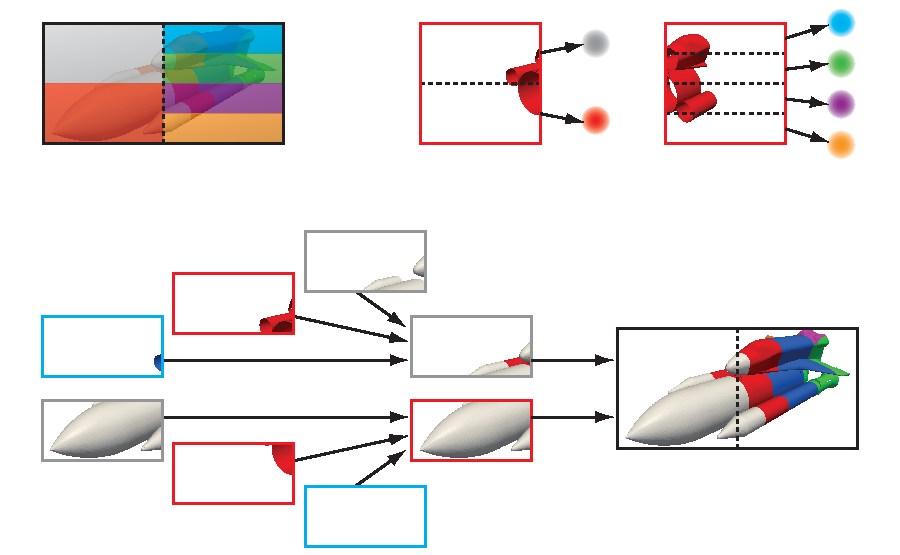
\includegraphics{images/TileSplit}
  \caption[Split strategy composite network.]{Compositing for split
    strategy.  First tiles are split and assigned to processes (upper
    left).  Then each process simultaneously sends its images to the
    responsible process (upper right) and receives all sub-images for its
    piece (bottom).  The composited pieces are then collected and stitched
    together.}
  \label{fig:TileSplit}
\end{figure}

The split strategy first assigns processes to tiles similar to how they are
assigned in the reduce strategy described previously.  That is, the number
of processes per tile is proportional to the number of non-empty images
generated for it.  Each tile is then split up evenly amongst all processes
assigned to it.  In the example in Figure~\ref{fig:TileSplit}, the upper
left image shows that the left image is split between 2 processes and the
right image is split amongst 4 processes.

On being assigned a section of tile, each process prepares to receive data
from all the sending processes using asynchronous receives.  Each process
then renders its images, splits them up, and sends the sub-images to the
corresponding process.  When a process is ready and as it receives data,
the incoming images are composited together.  Once all of the incoming
images are composited, the complete sub-image is sent to the display process
to be stitched together.

The split strategy does not support ordered compositing.  Using the split
strategy in color blending mode will fail.

\index{strategy!split|)}

\section{Virtual Trees Strategy}
\label{sec:Strategies:Vertial_Trees}

\index{strategy!virtual~trees|(}
\index{virtual~trees|see{strategy, virtual trees}}

The \keyterm{virtual trees strategy} is based on the binary tree
compositing algorithm, but performs multiple composites simultaneously to
regain some of the load balance lost in the original algorithm.  The
virtual trees strategy has nice regular communications, but still suffers
from some load imbalance, particularly when using fewer tiles and in later
stages of the algorithm.  The virtual trees strategy is selected by calling
\CFunc{icetStrategy} with the \CEnum{ICET\_STRATEGY\_VTREE} argument.

\begin{figure}
  \centering
  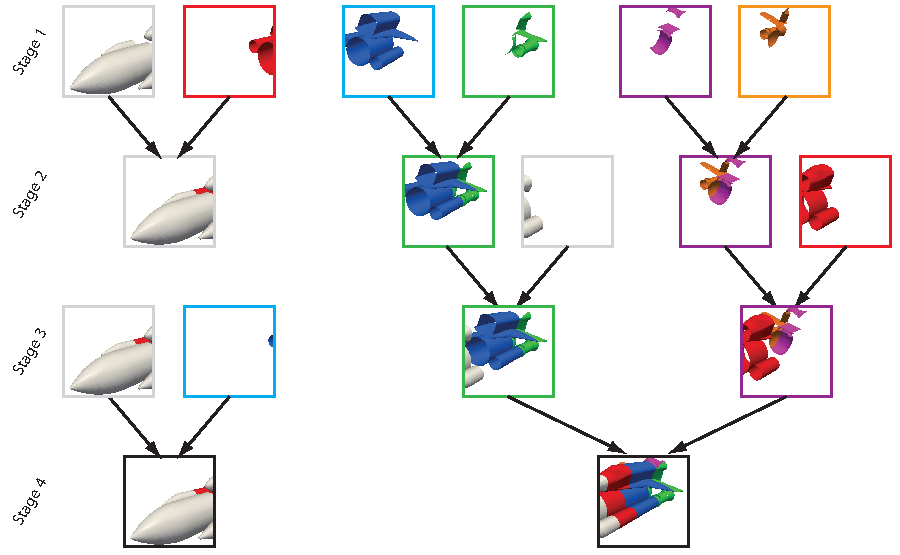
\includegraphics{images/VTrees}
  \caption[Virtual trees composite network.]{Composite network for virtual
    trees strategy.  Arrows represent the passing of data from one state to
    the next.  Processes receiving multiple images composite them
    together.}
  \label{fig:VTreesComposite}
\end{figure}

The virtual trees strategy works by creating a ``virtual'' tree for each
tile.  Contained in each tree are processes that have rendered an image for
that display tile.  The algorithm proceeds much like the binary tree
composition algorithm except that the processes float amongst the trees,
helping with the compositing as they become available.
Figure~\ref{fig:VTreesComposite} shows an example of the virtual trees
compositing.  In particular, notice that the gray process takes part in the
left tree in stage 1, then floats to take part in the right tree in stage
2, and then returns to take part in the left tree in stage 3.

When necessary, the process must keep track of multiple images belonging to
different virtual trees.  Two conserve memory, images are not rendered
until they are needed.  Also, a process can only hold two images at a time:
one that it is sending and one that it is receiving.  If a process is
holding an image for one tile, it cannot receive an image for another tile
until it sends away the image it is holding.

The virtual trees strategy does not support ordered compositing.  Using the
virtual trees strategy in color blending mode will fail.

\index{strategy!virtual~trees|)}

\section{Serial Strategy}
\label{sec:Strategies:Serial}

\index{strategy!serial|(}
\index{serial~strategy|see{strategy, serial}}

Despite its name, the \keyterm{serial strategy} does not completely
serialize the image compositing process.  Rather, it serially addresses the
tiles, but performs parallel compositing for each tile.  The serial
strategy is selected by calling \CFunc{icetStrategy} with the
\CEnum{ICET\_STRATEGY\_SERIAL} argument.

\begin{figure}
  \centering
  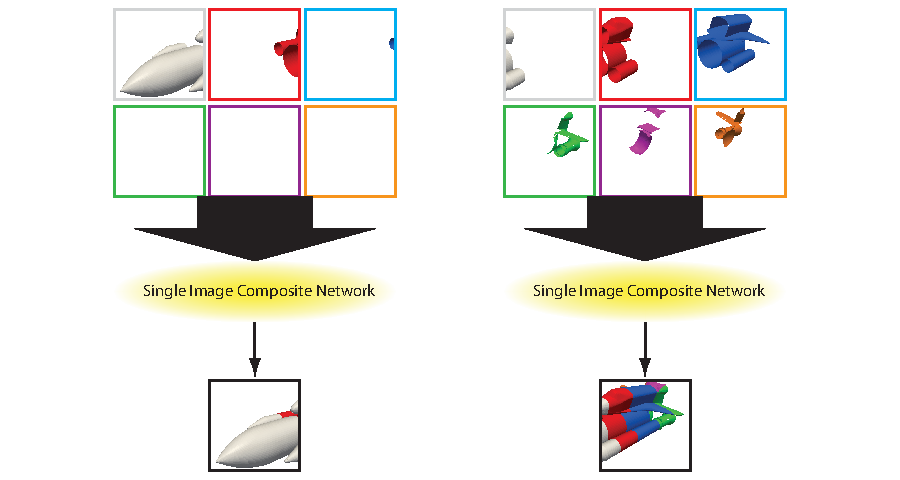
\includegraphics{images/SerialComposite}
  \caption[Serial compositing network.]{Composite network for serial
    compositing.  One at a time, each tile is composited using a parallel
    single image composite network described in a previous section.}
  \label{fig:SerialComposite}
\end{figure}

The serial strategy iterates over all of the tiles.  For each tile, it
composites all the images for that tile using one of the single image
compositing algorithms described in that preceding section.  As
demonstrated in the example in Figure~\ref{fig:SerialComposite} images from
all processes are composited for each tile regardless of whether some of
them may be empty.

Since the single image compositing algorithms support ordered
compositing, the serial strategy also supports ordered compositing.

The serial strategy is really only implemented as a baseline algorithm to
compare other algorithms.  In general, the reduce strategy does at least as
well or outperforms the serial strategy.  We have observed this even in
single tile mode, possibly because the reduce strategy can throw away empty
images.

\index{strategy!serial|)}

\section{Direct Send Strategy}
\label{sec:Strategies:DirectSend}

\index{strategy!direct~send|(}
\index{direct~send~strategy|see{strategy, direct send}}

The \keyterm{direct send strategy} is the simplest of all the strategies.
Each process simply renders its images and sends them directly to the
display process where the images get composited, as shown in
Figure~\ref{fig:DirectSend}.  The direct send strategy is selected by
calling \CFunc{icetStrategy} with the \CEnum{ICET\_STRATEGY\_DIRECT}
argument.

\begin{figure}
  \centering
  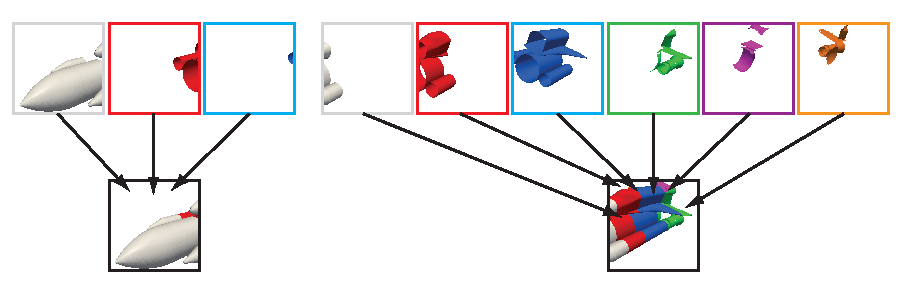
\includegraphics{images/DirectSend}
  \caption[Direct send compositing network.]{Composite network for direct
    send compositing.  Arrows represent the passing of data from one
    process to another.  Receiving process composite all incoming images
    together.}
  \label{fig:DirectSend}
\end{figure}

The direct send strategy is usually a poor performer.  It was designed as a
low watermark to compare to other compositing strategies.  The direct send
strategy does, however, support ordered compositing.

\index{strategy!direct~send|)}

\section{Implementing New Strategies}

\index{strategy|)}
